{
\usetikzlibrary{math}

\definecolor{c1}{RGB}{0, 114, 178}
\definecolor{c2}{RGB}{213, 94, 0}
\definecolor{c3}{RGB}{0, 158, 115}
\definecolor{c3prime}{RGB}{240, 228, 66}
\definecolor{b1}{RGB}{230, 159, 0}
\definecolor{b2}{RGB}{86, 180, 233}
\definecolor{b3}{RGB}{204, 121, 167}

% \colorlet{c1}{cyan}
% \colorlet{c2}{red}
% \colorlet{c3}{green}
% \colorlet{c3prime}{violet}
% \colorlet{b1}{brown}
% \colorlet{b2}{olive}
% \colorlet{b3}{gray}

\begin{figure}[t]
    \centering
    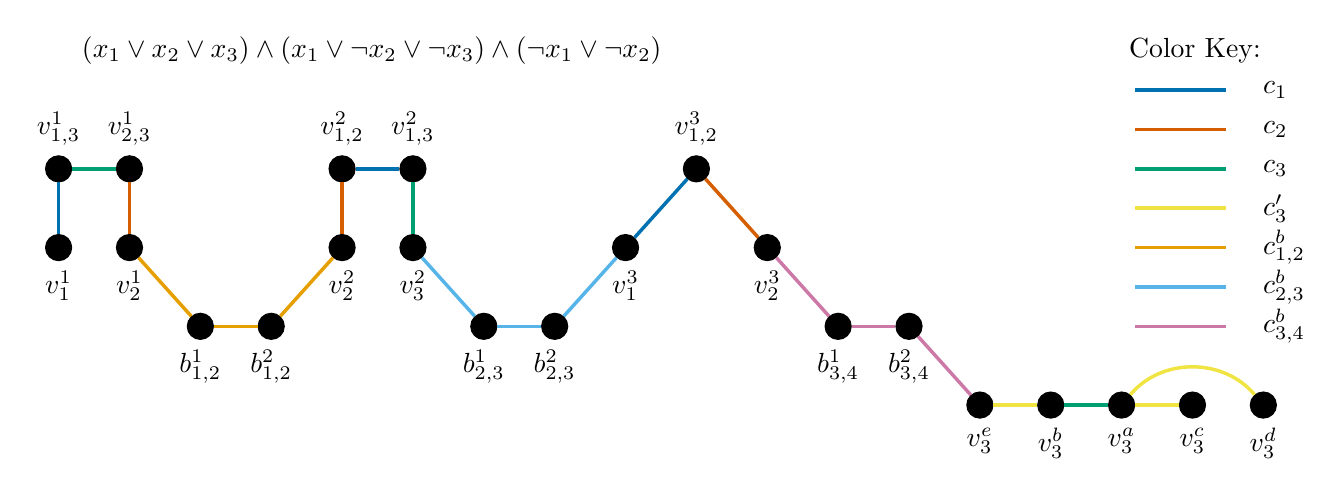
\begin{tikzpicture}

        \tikzmath{
            \leftx = 0;
            \dy = 1;
            \confy = 0;
            \freey = \confy - \dy;
            \bridgey = \confy - 2*\dy;
            \sparey = \confy - 3*\dy;
            \dx = .9;
            \edgewidth = 1.25;
            \keyx = \leftx + 15*\dx;
            \keyy = \confy + 1.5;
            \keydx = 1.5;
            \keydy = -.5;
            \keytitlex = \keyx-.2;}

        \node[circle, label=right:$(x_1 \lor x_2 \lor x_3) \land (x_1 \lor \neg x_2 \lor \neg x_3) \land (\neg x_1 \lor \neg x_2)$] at (\leftx, \keyy) (formula) {};

        \node[circle, draw, fill=black, label=below:$v_1^1$] at (\leftx, \freey) (free11) {};
        \node[circle, draw, fill=black, label=above:$v_{1,3}^1$] at (\leftx, \confy) (conf131) {};
        \node[circle, draw, fill=black, label=above:$v_{2,3}^1$] at (\leftx + \dx, \confy) (conf231) {};
        \node[circle, draw, fill=black, label=below:$v_2^1$] at (\leftx + \dx, \freey) (free21) {};

        \draw[c1, line width=\edgewidth pt] (free11) -- (conf131);
        \draw[c3, line width=\edgewidth pt] (conf131) -- (conf231);
        \draw[c2, line width=\edgewidth pt] (conf231) -- (free21);

        \node[circle, draw, fill=black, label=below:$b_{1,2}^1$] at (\leftx + 2*\dx, \bridgey) (bridge121) {};
        \node[circle, draw, fill=black, label=below:$b_{1,2}^2$] at (\leftx + 3*\dx, \bridgey) (bridge122) {};

        \node[circle, draw, fill=black, label=below:$v_2^2$] at (\leftx + 4*\dx, \freey) (free22) {};
        \node[circle, draw, fill=black, label=above:$v_{1,2}^2$] at (\leftx + 4*\dx, \confy) (conf122) {};
        \node[circle, draw, fill=black, label=above:$v_{1,3}^2$] at (\leftx + 5*\dx, \confy) (conf132) {};
        \node[circle, draw, fill=black, label=below:$v_3^2$] at (\leftx + 5*\dx, \freey) (free32) {};

        \draw[c2, line width=\edgewidth pt] (free22) -- (conf122);
        \draw[c1, line width=\edgewidth pt] (conf122) -- (conf132);
        \draw[c3, line width=\edgewidth pt] (conf132) -- (free32);

        \node[circle, draw, fill=black, label=below:$b_{2,3}^1$] at (\leftx + 6*\dx, \bridgey) (bridge231) {};
        \node[circle, draw, fill=black, label=below:$b_{2,3}^2$] at (\leftx + 7*\dx, \bridgey) (bridge232) {};

        \node[circle, draw, fill=black, label=below:$v_1^3$] at (\leftx + 8*\dx, \freey) (free13) {};
        \node[circle, draw, fill=black, label=above:$v_{1,2}^3$] at (\leftx + 9*\dx, \confy) (conf123) {};
        \node[circle, draw, fill=black, label=below:$v_2^3$] at (\leftx + 10*\dx, \freey) (free23) {};

        \draw[c1, line width=\edgewidth pt] (free13) -- (conf123);
        \draw[c2, line width=\edgewidth pt] (conf123) -- (free23);

        \node[circle, draw, fill=black, label=below:$b_{3,4}^1$] at (\leftx + 11*\dx, \bridgey) (bridge341) {};
        \node[circle, draw, fill=black, label=below:$b_{3,4}^2$] at (\leftx + 12*\dx, \bridgey) (bridge342) {};

        \node[circle, draw, fill=black, label=below:$v_3^e$] at (\leftx + 13*\dx, \sparey) (spare3e) {};
        \node[circle, draw, fill=black, label=below:$v_3^b$] at (\leftx + 14*\dx, \sparey) (spare3b) {};
        \node[circle, draw, fill=black, label=below:$v_3^a$] at (\leftx + 15*\dx, \sparey) (spare3a) {};
        \node[circle, draw, fill=black, label=below:$v_3^c$] at (\leftx + 16*\dx, \sparey) (spare3c) {};
        \node[circle, draw, fill=black, label=below:$v_3^d$]     at (\leftx + 17*\dx, \sparey) (spare3d) {};

        \draw[c3prime, line width=\edgewidth pt] (spare3e) -- (spare3b);
        \draw[c3, line width=\edgewidth pt] (spare3b) -- (spare3a);
        \draw[c3prime, line width=\edgewidth pt] (spare3a) -- (spare3c);
        \draw[c3prime, line width=\edgewidth pt] (spare3a) to[bend left=50] (spare3d);
    
        
        \draw[b1, line width=\edgewidth pt] (free21) -- (bridge121);
        \draw[b1, line width=\edgewidth pt] (bridge121) -- (bridge122);
        \draw[b1, line width=\edgewidth pt] (bridge122) -- (free22);

        \draw[b2, line width=\edgewidth pt] (free32) -- (bridge231);
        \draw[b2, line width=\edgewidth pt] (bridge231) -- (bridge232);
        \draw[b2, line width=\edgewidth pt] (bridge232) -- (free13);

        \draw[b3, line width=\edgewidth pt] (free23) -- (bridge341);
        \draw[b3, line width=\edgewidth pt] (bridge341) -- (bridge342);
        \draw[b3, line width=\edgewidth pt] (bridge342) -- (spare3e);


        \node[circle, label=right:{Color Key:}] at (\keytitlex, \keyy) () {};

        \node[circle] at (\keyx, \keyy + \keydy) (c1left) {};
        \node[circle, label=right:$c_1$] at (\keyx + \keydx, \keyy + \keydy) (c1right) {};
        \draw[c1, line width=\edgewidth pt] (c1left) -- (c1right);

        \node[circle] at (\keyx, \keyy + 2*\keydy) (c1left) {};
        \node[circle, label=right:$c_2$] at (\keyx + \keydx, \keyy + 2*\keydy) (c1right) {};
        \draw[c2, line width=\edgewidth pt] (c1left) -- (c1right);

        \node[circle] at (\keyx, \keyy + 3*\keydy) (c1left) {};
        \node[circle, label=right:$c_3$] at (\keyx + \keydx, \keyy + 3*\keydy) (c1right) {};
        \draw[c3, line width=\edgewidth pt] (c1left) -- (c1right);

        \node[circle] at (\keyx, \keyy + 4*\keydy) (c1left) {};
        \node[circle, label=right:$c_3'$] at (\keyx + \keydx, \keyy + 4*\keydy) (c1right) {};
        \draw[c3prime, line width=\edgewidth pt] (c1left) -- (c1right);

        \node[circle] at (\keyx, \keyy + 5*\keydy) (c1left) {};
        \node[circle, label=right:$c_{1,2}^b$] at (\keyx + \keydx, \keyy + 5*\keydy) (c1right) {};
        \draw[b1, line width=\edgewidth pt] (c1left) -- (c1right);

        \node[circle] at (\keyx, \keyy + 6*\keydy) (c1left) {};
        \node[circle, label=right:$c_{2,3}^b$] at (\keyx + \keydx, \keyy + 6*\keydy) (c1right) {};
        \draw[b2, line width=\edgewidth pt] (c1left) -- (c1right);

        \node[circle] at (\keyx, \keyy + 7*\keydy) (c1left) {};
        \node[circle, label=right:$c_{3,4}^b$] at (\keyx + \keydx, \keyy + 7*\keydy) (c1right) {};
        \draw[b3, line width=\edgewidth pt] (c1left) -- (c1right);
    \end{tikzpicture}
    \caption{\label{fig:hardness} The construction given by~\Cref{thm:cfminecc-NPhard} for the CNF formula on three clauses $C_1 = (x_1 \lor x_2 \lor x_3)$, $C_2 = (x_1 \lor \neg x_2 \lor \neg x_3)$, and $C_3 = (\neg x_1 \lor \neg x_2)$. 
    Notice that the vertices are partitioned visually into four horizontal layers. The top layer contains \emph{conflict} vertices, the second from top contains \emph{free} vertices, the second from bottom \emph{bridge} vertices, and the bottom \emph{spare} vertices.
    Every edge containing a conflict vertex is a \emph{conflict} edge, every edge containing a bridge vertex is a \emph{bridge} edge, and all other edges are \emph{spare} edges.
    The colors $c_1, c_2$ and $c_3$ correspond to the clauses $C_1, C_2$, and $C_3$. The color $c_3'$ is the \emph{spare} color associated with $C_3$. The remaining colors are \emph{bridge} colors. We refer to the proof of~\Cref{thm:cfminecc-NPhard} for a formal description of the construction and the accompanying analysis.
    }

\end{figure}
}